\vspace{-2mm}
 \section{Experiments}\label{sec:experiment}
\vspace{-2mm}
 We conduct experiments to assess the performance of our algorithm relative to baselines and its sensitivity to various hyperparameters. We start by outlining the experimental setup, including baselines and models, and then present the results.

\vspace{-2mm}
\subsection{Settings}
\vspace{-2mm}



{ \paragraph{Methods to compare.} 
We compare \alg\ to several representative methods capable of performing reward maximization during inference, discussed in \pref{sec:related_works}.   
\vspace{-2mm}
\begin{itemize}[leftmargin=*] 
    \item \textbf{Pre-trained models:} We generate samples using pre-trained models.
    \item \textbf{Best-of-N:} We generate samples from pre-trained models and select the top $1/N$ samples. This selection is made to ensure that the computational time during inference is approximately equivalent to that of \alg. 
    \item \textbf{DPS \citep{chung2022diffusion}:} It is a widely used training-free version of classifier guidance. For discrete diffusion, we combine it with the state-of-the-art approach \citep{nisonoff2024unlocking}.
    \item \textbf{SMC-Based Methods (SMC):} Methods discussed in \pref{sec:TDS} and Appendix~\ref{sec:filter}, which do not require differentiable models, like \alg. 
    \item \textbf{\alg\,(Ours):} We implement \alg-MC and \alg-PM. We generally set $M=20$ for images and $M=10$ for other domains, and $\alpha =0$. Recall $M$ is the duplication size in the IS part. %
\end{itemize}} 

\vspace{-2mm}
\paragraph{Datasets and reward models. } We provide details on the pre-trained diffusion models and downstream reward functions used. For further information, refer to \pref{sec:additional}. 

\vspace{-2mm}
\begin{itemize}[leftmargin=*]
    \item \textbf{Images}: We use Stable Diffusion v1.5 as the pre-trained diffusion model ($T=50$). For downstream reward functions, we use compressibility and aesthetic scores (LAION Aesthetic Predictor V2 in \citet{schuhmann2022laion}), as employed by \citet{black2023training,fan2023dpok}. Compressibility is a \emph{non-differentiable reward feedback}.
    \item \textbf{Molecules}:  We use GDSS \citep{jo2022score}, trained on ZINC-250k \citep{irwin2005zinc}, as the pre-trained diffusion model ($T=1000$). For downstream reward functions, we use drug-likeness (QED) and synthetic accessibility (SA) calculated by RDKit, as well as docking score (DS) calculated by QuickVina 2 \citep{alhossary2015fast}, which are all \emph{non-differentiable feedback}. Here, we renormalize SA to $(10 - \mathrm{SA}) / 9$ and docking score to $\max(-\mathrm{DS}, 0)$, so that a higher value indicates better performance. The docking scores measure binding affinity regarding four target proteins: Parp1, 5ht1b, Jak2, and Braf following~\cite{yang2021hit}. These tasks are critical for drug discovery. 
    \item \textbf{DNAs (enhancers) and RNAs (5'Untranslated regions (UTRs))}: We use the discrete diffusion model \citep{sahoo2024simple}, trained on datasets from \citet{gosai2023machine} for enhancers, and from  \citet{sample2019human} for 5'UTRs, as our pre-trained diffusion model ($T=128$). For the reward functions, we use an Enformer model \citep{avsec2021effective} to predict activity of enhancers in the HepG2 cell line, and a ConvGRU model that predicts the mean ribosomal load (MRL) of 5'UTRs measured by polysome profiling, respectively \citep{sample2019human}. 
These tasks are highly relevant for cell and RNA therapies, respectively \citep{taskiran2024cell,castillo2021machine}. 
\end{itemize} 

\vspace{-2mm}
\subsection{Results}
\vspace{-2mm}

{
\begin{table}[!ht]
    \centering  
    \setlength{\belowcaptionskip}{-6pt}
    \caption{Top 10 and 50 quantiles of the generated samples for each algorithm (with 95\% confidence intervals). Higher is better. \alg\ consistently outperforms the baseline methods. }
    \resizebox{\textwidth}{!}{
    \label{tab:important}
    \begin{tabular}{c|c|ccccgg} \toprule 
       Domain  & Quantile & Pre-Train & Best-N & DPS  & SMC & \textbf{\alg-MC} & \textbf{\alg-PM}    \\   \midrule  
Image: Compress & 50\%  & -101.4 $\pm$  0.22 & -71.2 $\pm$  0.46  &   -60.1 $\pm$  0.44  &  -59.7 $\pm$  0.4 & -54.3 $\pm$  0.33 & \textbf{-51.1} $\pm$  0.38 \\ 
& 10\%  & -78.6 $\pm$ 0.13 & -57.3 $\pm$ 0.28 &  -61.2 $\pm$ 0.28 &   -49.9 $\pm$ 0.24  &   -40.4 $\pm$ 0.2 & \textbf{-38.8} $\pm$ 0.23 \\ \midrule 
Image: Aesthetic & 50\%  & 5.62 $\pm$ 0.003 & 6.11 $\pm$ 0.007 & 5.61 $\pm$ 0.009 & 6.02 $\pm$ 0.004 & 5.70 $\pm$ 0.008 & \textbf{6.14} $\pm$ 0.007\\ 
  & 10\%  &  5.98 $\pm$ 0.002 &  6.34 $\pm$ 0.004&  6.00 $\pm$ 0.005 & 6.28 $\pm$ 0.003 & 6.05 $\pm$ 0.005 & \textbf{6.47} $\pm$ 0.004 \\  \midrule 
     Molecule: QED & 50\% & 0.656 $\pm$ 0.008 & 0.835 $\pm$ 0.009 & 0.679 $\pm$ 0.024 &  0.667 $\pm$ 0.016 & \textbf{0.852} $\pm$ 0.011 & {0.848} $\pm$ 0.014 \\
& 10\% & 0.812 $\pm$ 0.005 & 0.902 $\pm$ 0.006 & 0.842 $\pm$ 0.014 &  0.722 $\pm$ 0.009 & 0.925 $\pm$ 0.007 & \textbf{0.928} $\pm$ 0.008 \\  \midrule 
Molecule: SA   & 50\% & 0.652 $\pm$ 0.007 & 0.834 $\pm$ 0.014 & 0.693 $\pm$ 0.022 &  0.786 $\pm$ 0.004 & \textbf{0.935} $\pm$ 0.010 & 0.925 $\pm$ 0.016 \\
& 10\% & 0.803 $\pm$ 0.004 & 0.941 $\pm$ 0.008 & 0.844 $\pm$ 0.013 &  0.796 $\pm$ 0.003 & \textbf{1.000} $\pm$ 0.006 & \textbf{1.000} $\pm$ 0.010 \\  \midrule 
 Molecule: Docking parp1 & 50\% & 7.15 $\pm$ 0.52 & 10.00 $\pm$ 0.17 & 7.35 $\pm$ 0.43 & 6.90 $\pm$ 0.60 & \textbf{12.00} $\pm$ 0.26 & 11.40 $\pm$ 0.22 \\
& 10\% & 8.59 $\pm$ 0.31 & 10.67 $\pm$ 0.10 & 9.31 $\pm$ 0.26 & 9.37 $\pm$ 0.36 & \textbf{13.25} $\pm$ 0.16 & 12.41 $\pm$ 0.13 \\ \midrule 
 Molecule: Docking 5ht1b  & 50\% & 7.20 $\pm$ 0.53 & 9.65 $\pm$ 0.17 & 7.30 $\pm$ 0.48 & 6.80 $\pm$ 0.35 & \textbf{10.50} $\pm$ 0.46 & \textbf{10.50} $\pm$ 0.53 \\
& 10\% & 8.69 $\pm$ 0.32 & 10.28 $\pm$ 0.10 & 9.21 $\pm$ 0.29 & 9.00 $\pm$ 0.21 & \textbf{12.87} $\pm$ 0.28 & 12.30 $\pm$ 0.32 \\ \midrule
Molecule: Docking jak2 & 50\% & 7.05 $\pm$ 0.45 & 8.85 $\pm$ 0.17 & 7.30 $\pm$ 0.43 & 6.80 $\pm$ 0.46 & \textbf{10.65} $\pm$ 0.35 & 10.30 $\pm$ 0.45 \\
& 10\% & 8.20 $\pm$ 0.27 & 9.59 $\pm$ 0.10 & 8.70 $\pm$ 0.26 & 10.00 $\pm$ 0.28 & 11.80 $\pm$ 0.21 & \textbf{11.91} $\pm$ 0.27 \\ \midrule
Molecule: Docking braf & 50\% & 7.20 $\pm$ 0.40 & 9.20 $\pm$ 0.11 & 7.50 $\pm$ 0.23 & 6.90 $\pm$ 0.46 & \textbf{10.00} $\pm$ 0.37 & 9.65 $\pm$ 0.33 \\
& 10\% & 8.59 $\pm$ 0.24 & 10.29 $\pm$ 0.07 & 9.20 $\pm$ 0.14 & 8.74 $\pm$ 0.28 & 11.30 $\pm$ 0.22 & \textbf{11.40} $\pm$ 0.20 \\ \midrule
  Enhancers & 50\% & 0.121 $\pm$ 0.033 & 1.807 $\pm$ 0.214 & 3.782 $\pm$ 0.299 &  $4.28\pm 0.02$ & 5.074 $\pm$ 0.096 & \textbf{5.353} $\pm$ 0.231 \\
& 10\% & 1.396 $\pm$ 0.020 & 3.449 $\pm$ 0.128 & 4.879 $\pm$ 0.179 & $5.95\pm 0.01$ & 5.639 $\pm$ 0.057 & \textbf{6.980} $\pm$ 0.138 \\ \midrule 
5'UTR & 50\% & 0.406 $\pm$ 0.028 & 0.912 $\pm$ 0.023 & 0.426 $\pm$ 0.073 & $0.76\pm 0.02$ & 1.042 $\pm$ 0.008 & \textbf{1.214} $\pm$ 0.016 \\
& 10\% & 0.869 $\pm$ 0.017 & 1.064 $\pm$ 0.014 & 0.981 $\pm$ 0.044 & $0.91\pm 0.01$ & 1.117 $\pm$ 0.005 & \textbf{1.383} $\pm$ 0.010 \\
\bottomrule
    \end{tabular}
}
\end{table}



\begin{figure}[!th]
    \centering
    \subcaptionbox{Images: compressibility}{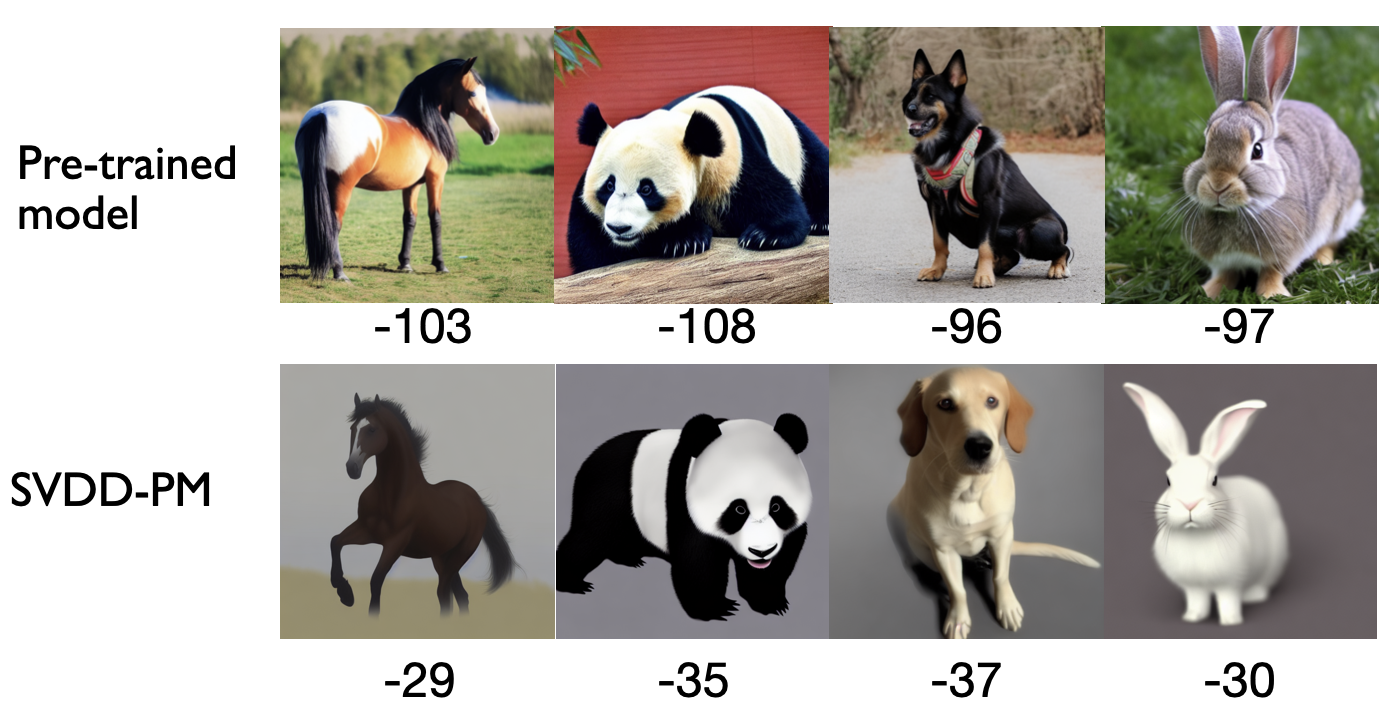
\includegraphics[width=.32\linewidth]{images/generated_images_comp.png}
    \label{fig:image}}
    \subcaptionbox{Images: aesthetic scores}{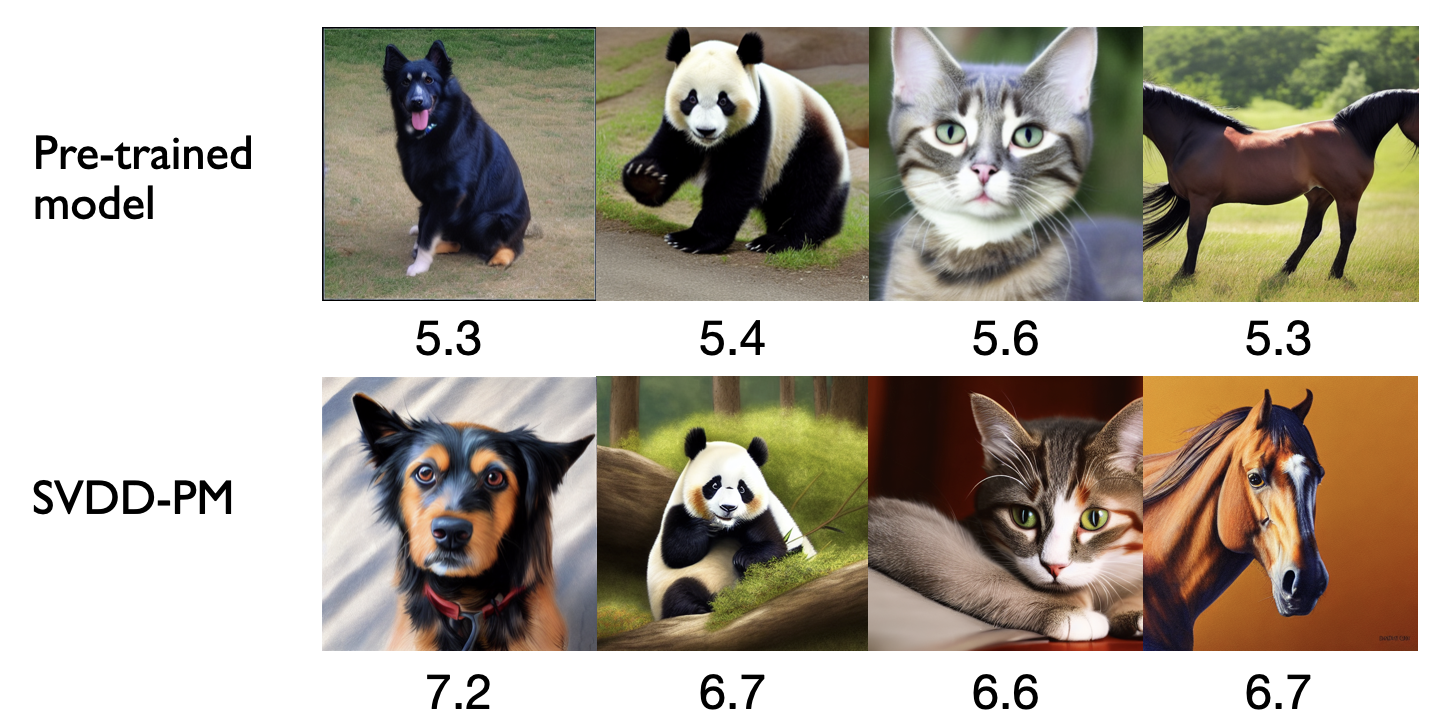
\includegraphics[width=.32\linewidth]{images/generated_images_asthetic.png}
    \label{fig:image2}}\\
    \subcaptionbox{Molecules: QED scores}{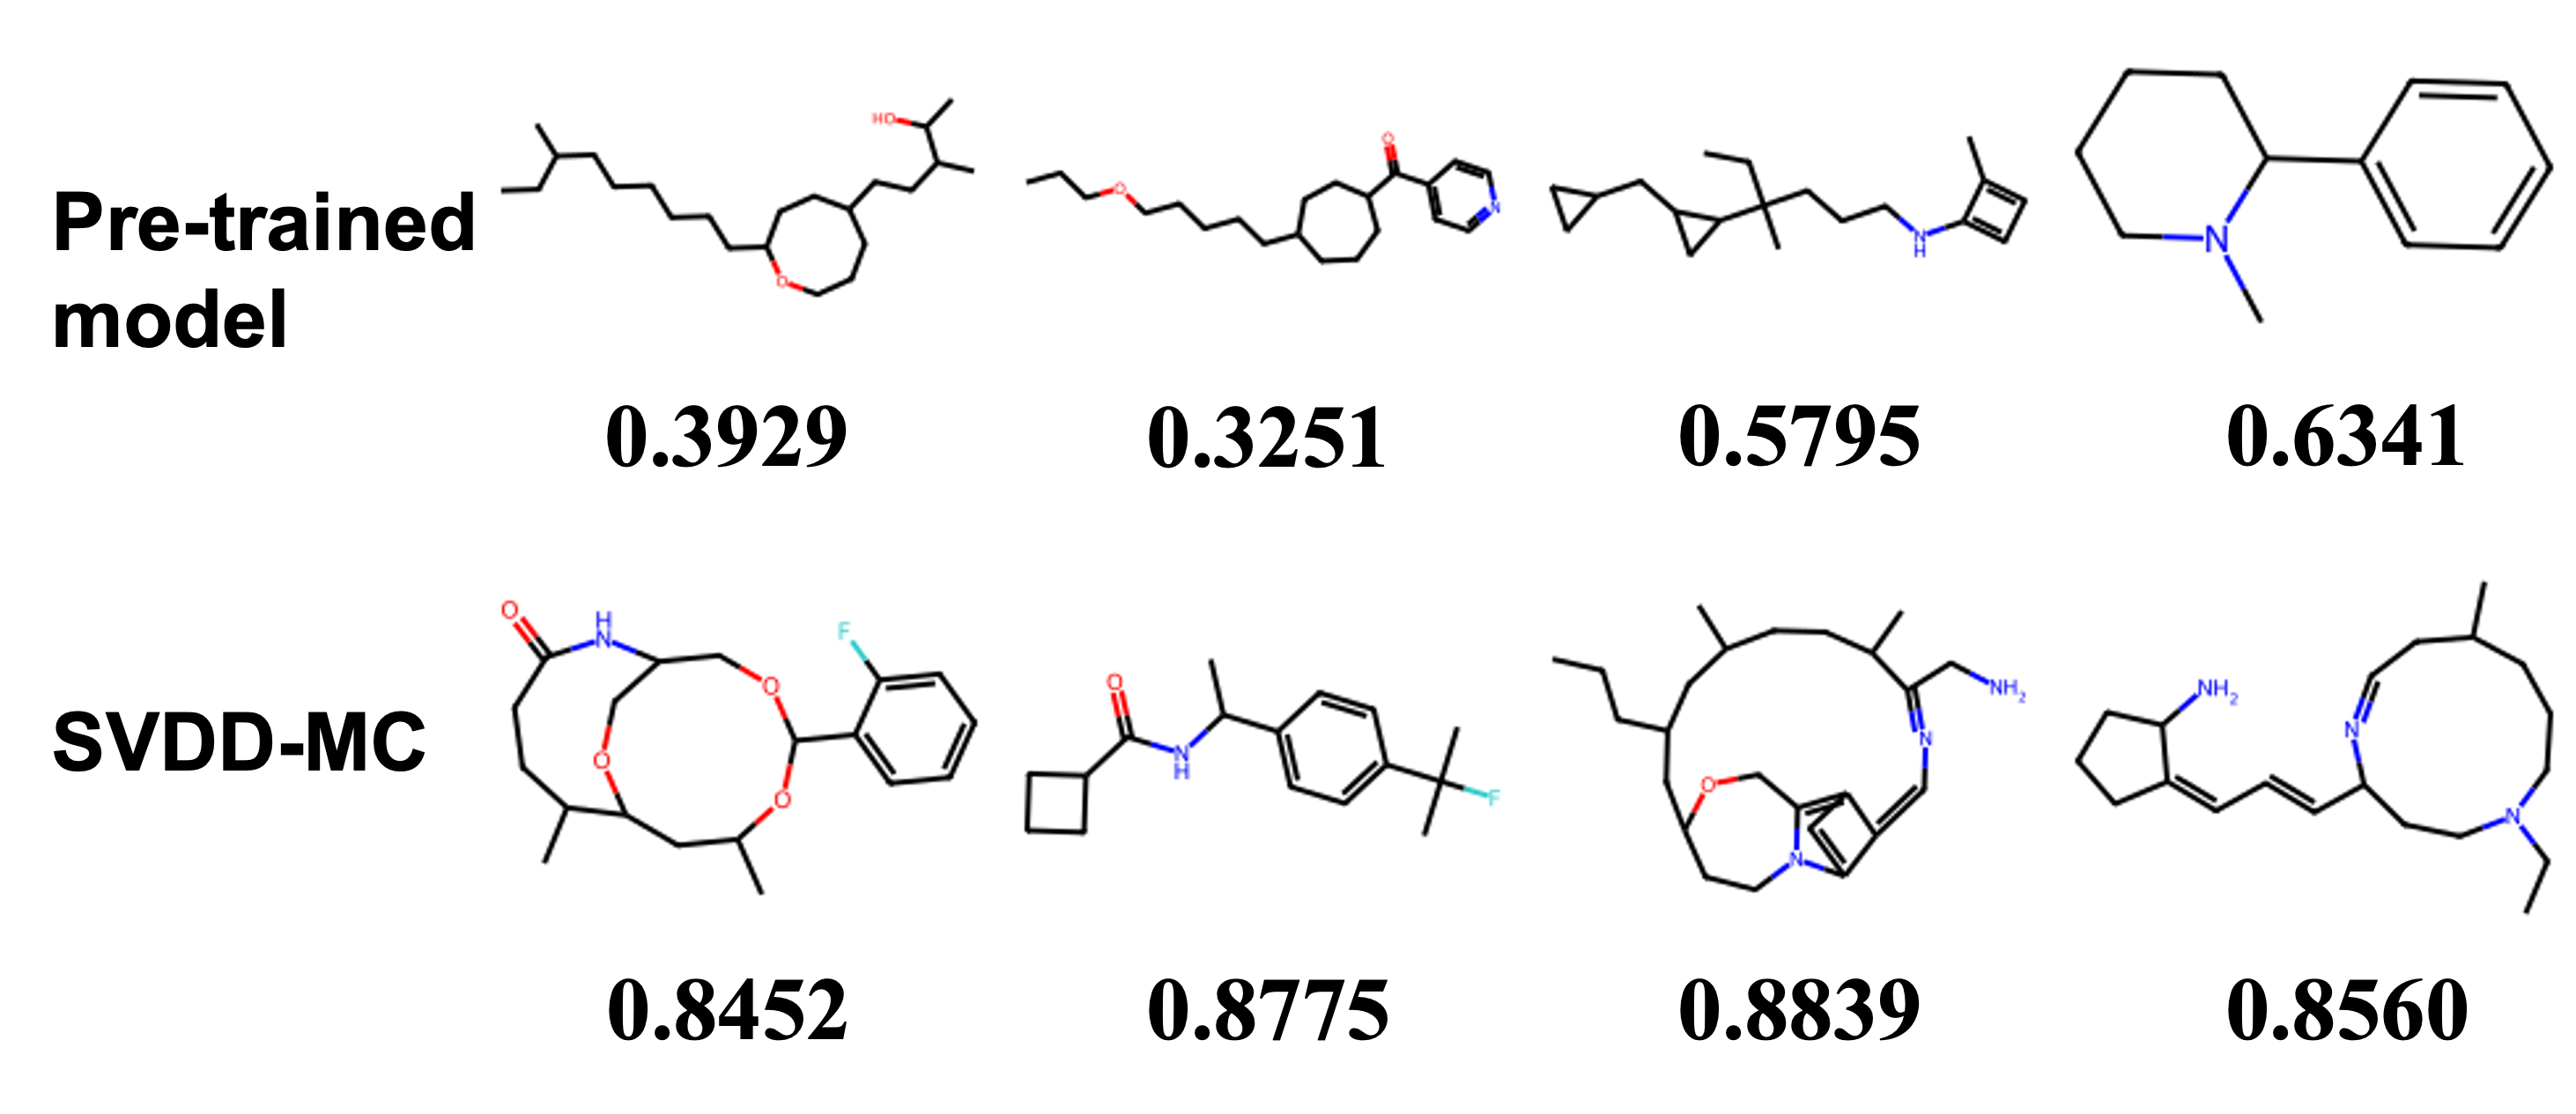
\includegraphics[width=.31\linewidth]{images/qed_grid.png}
    \label{fig:qed_grid}}
    \subcaptionbox{Molecules: SA scores (Normalized as $(10-SA)/9$ ) }{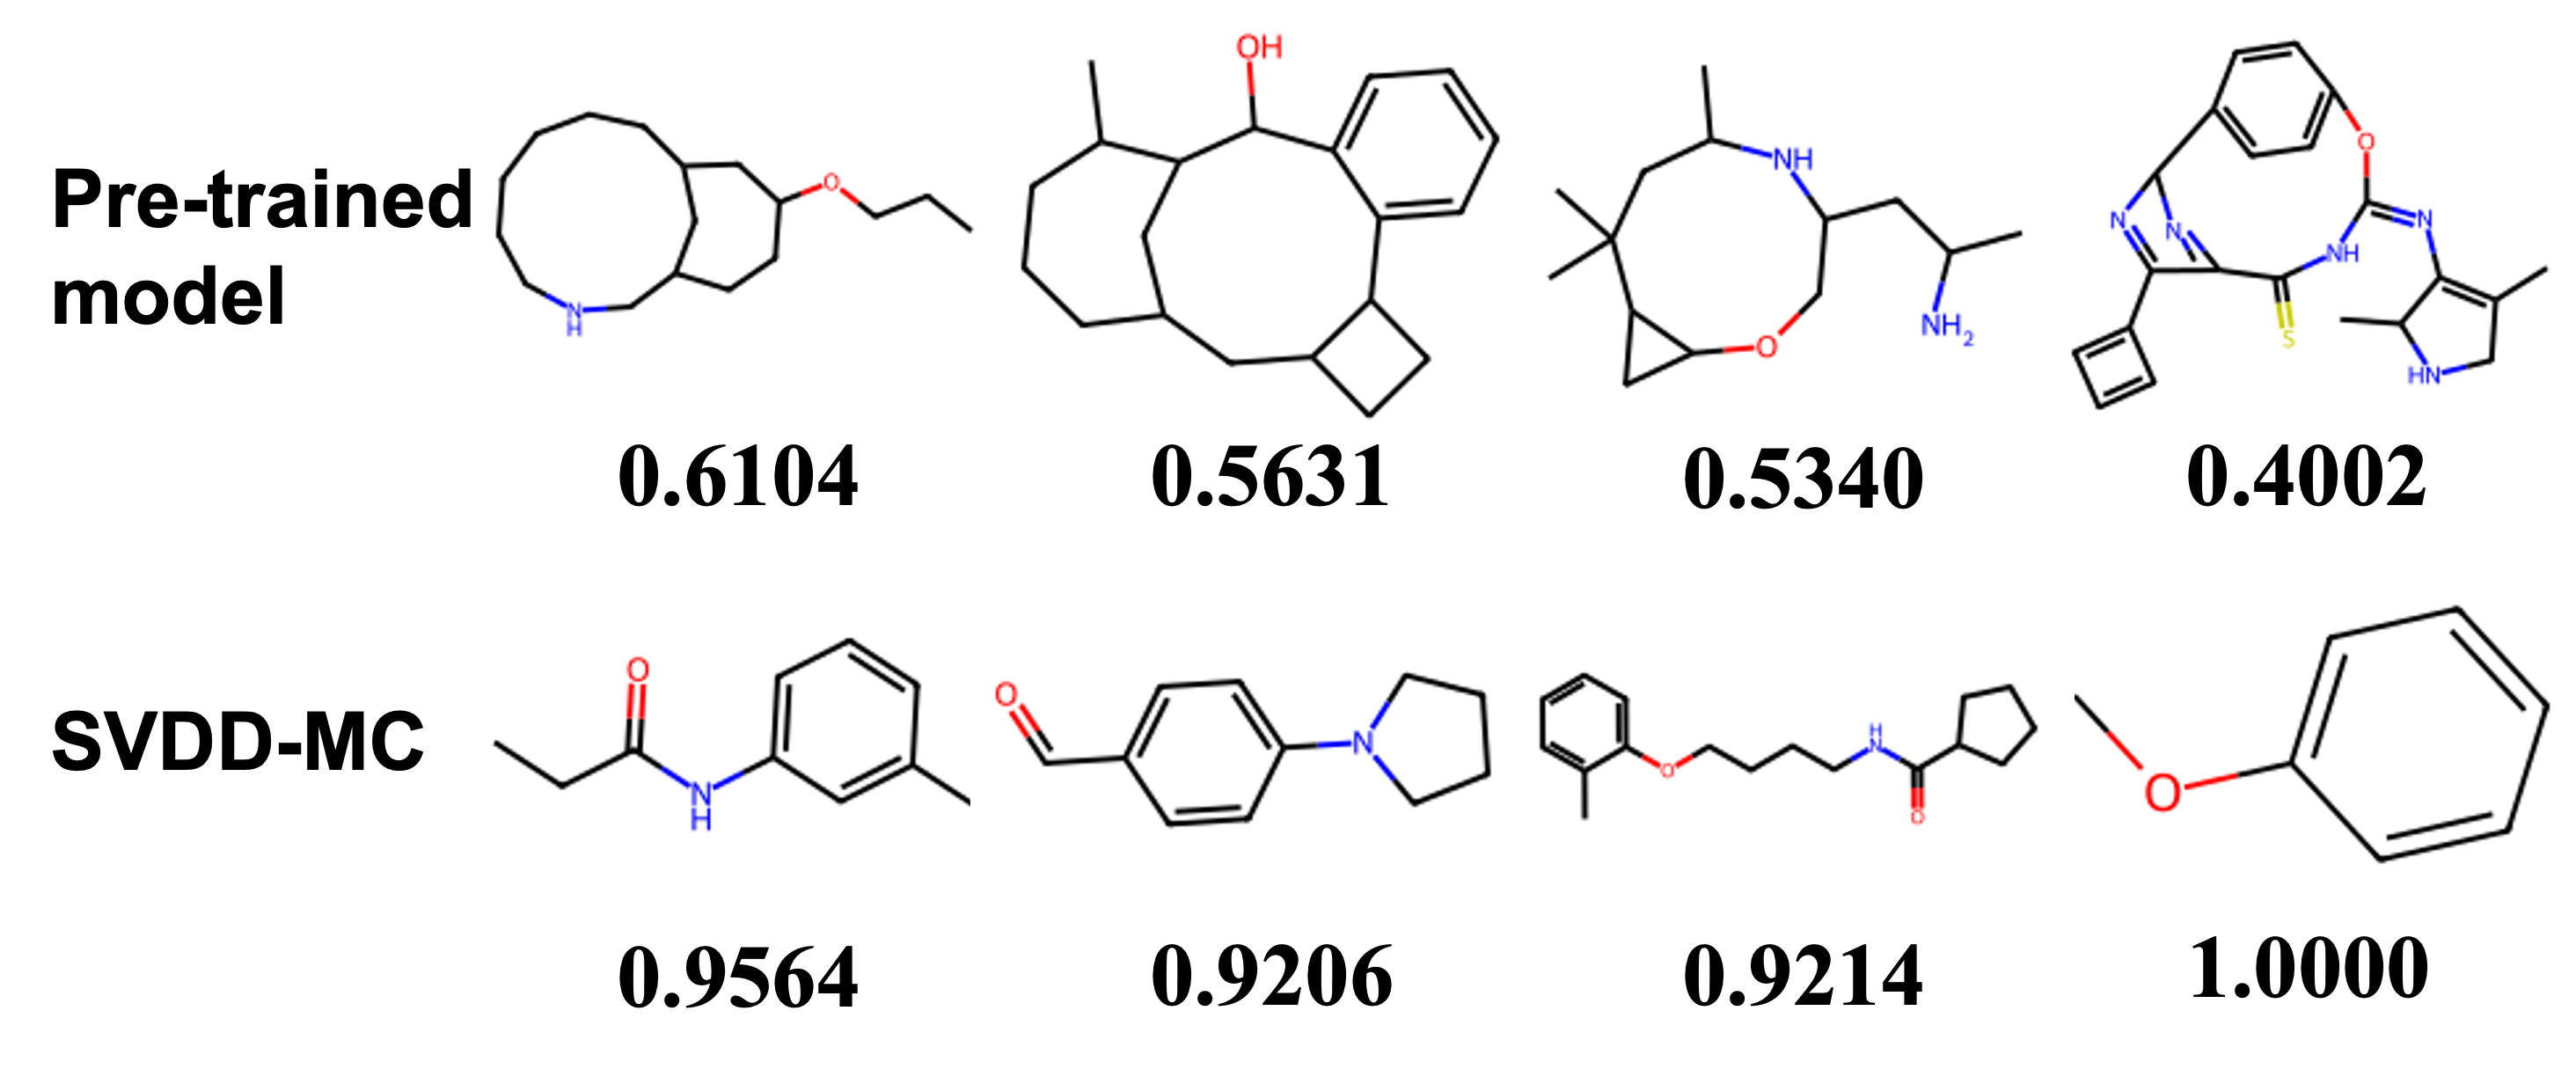
\includegraphics[width=.31\linewidth]{images/sa_grid.png}
    \label{fig:sa_grid}}
      \subcaptionbox{Molecules (by SVDD): high docking scores to Parp1 }{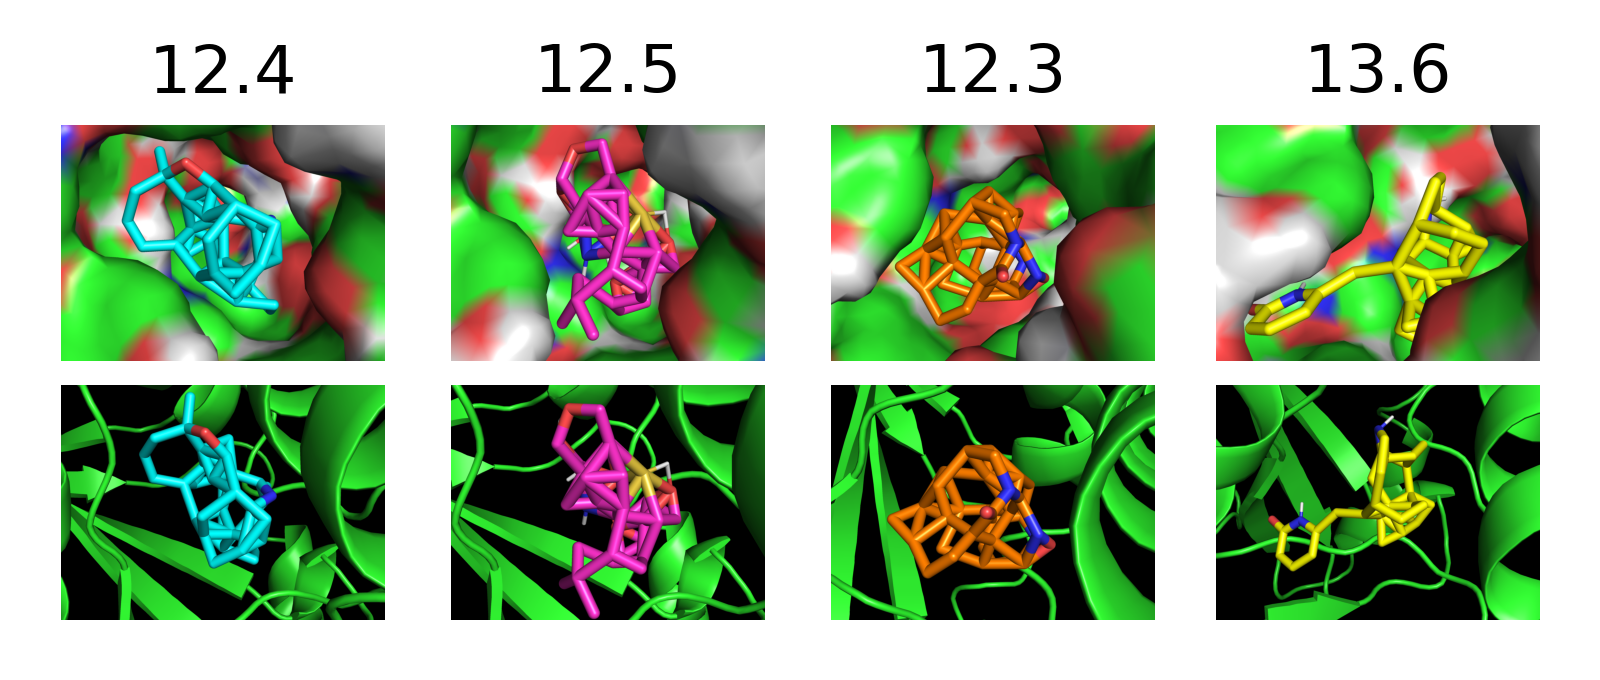
\includegraphics[width=.31\linewidth]{images/mol_vina1.png}
    \label{fig:vina1_grid}}
      \subcaptionbox{Molecules (by SVDD): high docking scores to 5ht1b  }{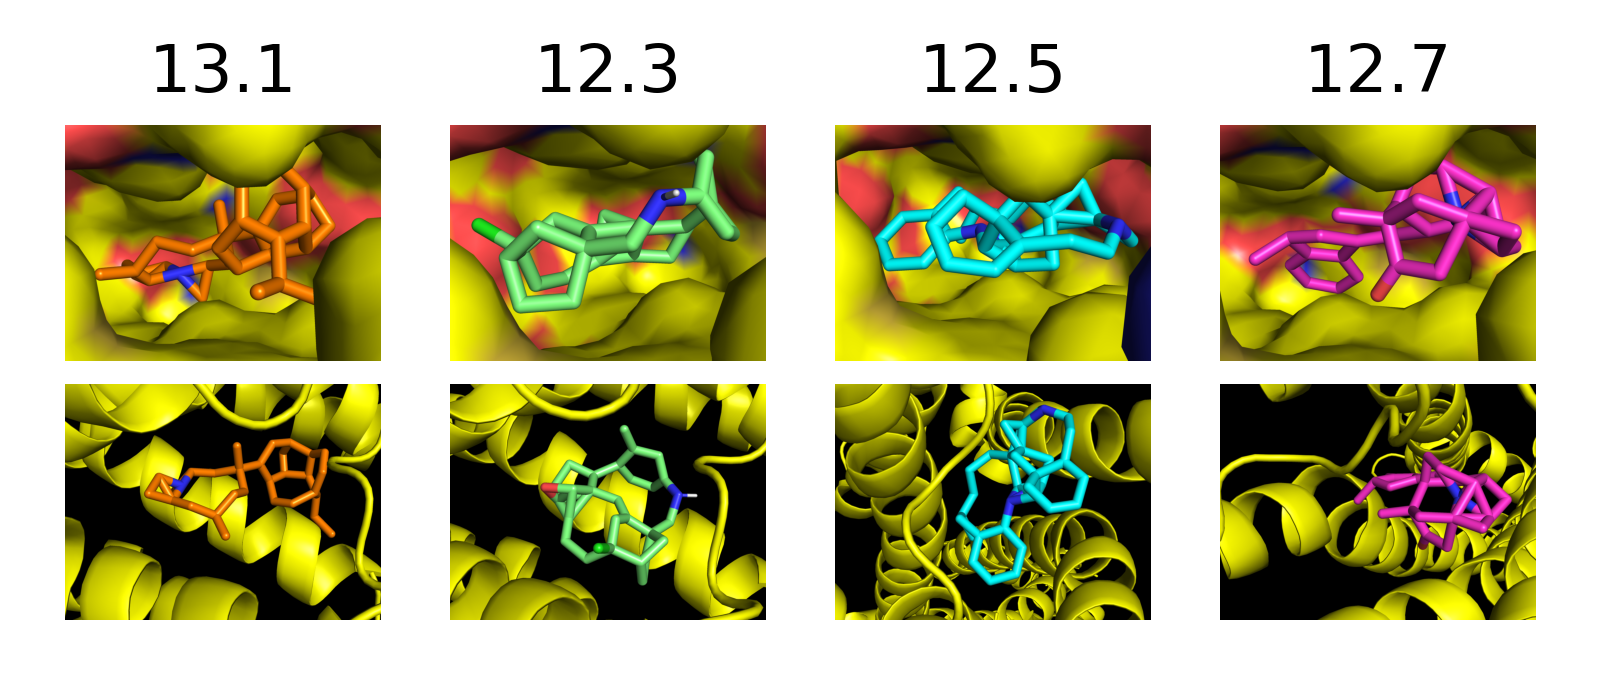
\includegraphics[width=.31\linewidth]{images/mol_vina3.png}
    \label{fig:vina3_grid}}
    \subcaptionbox{Molecules (by SVDD): high docking scores to Jak2 }{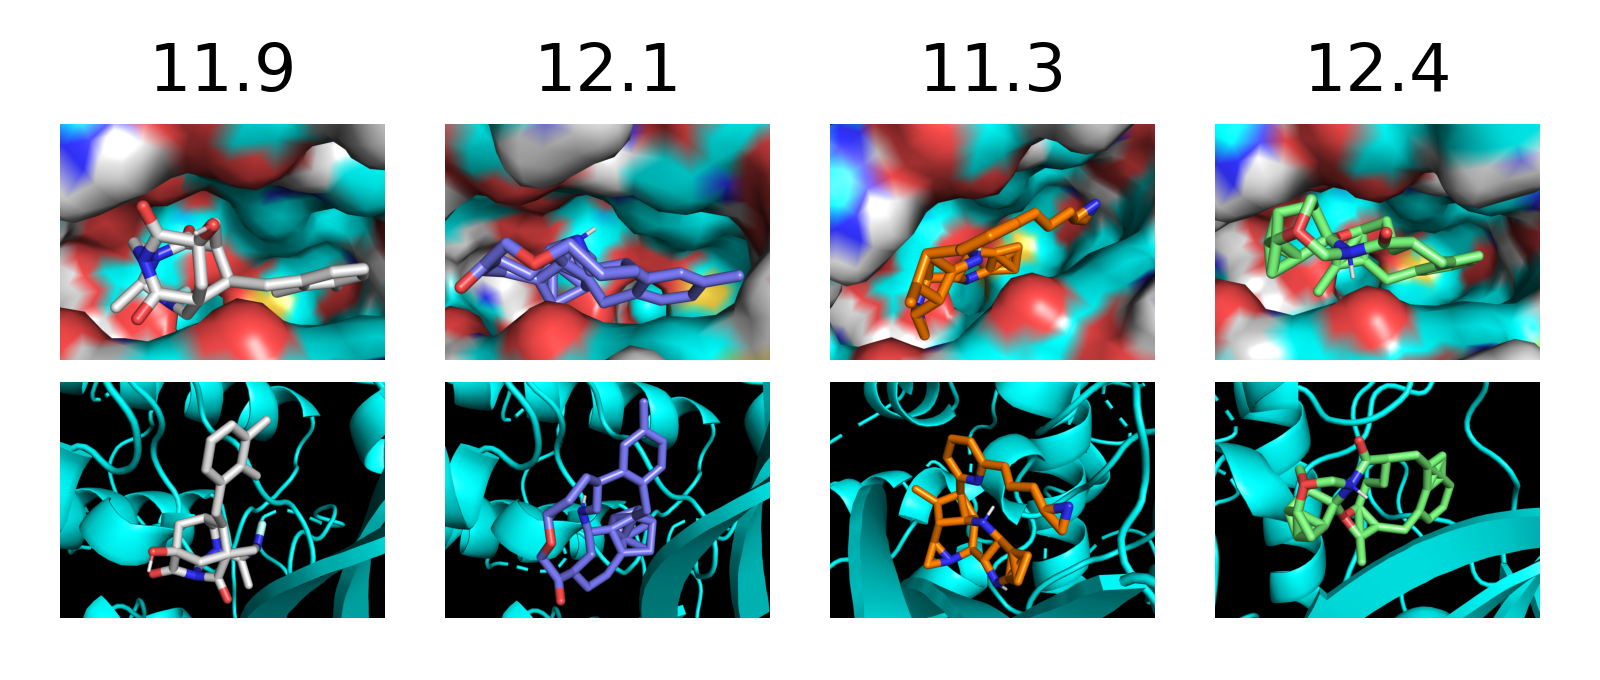
\includegraphics[width=.31\linewidth]{images/mol_vina4.png}
    \label{fig:vina4_grid}}
      \subcaptionbox{Molecules (by SVDD): high docking scores to Braf  }{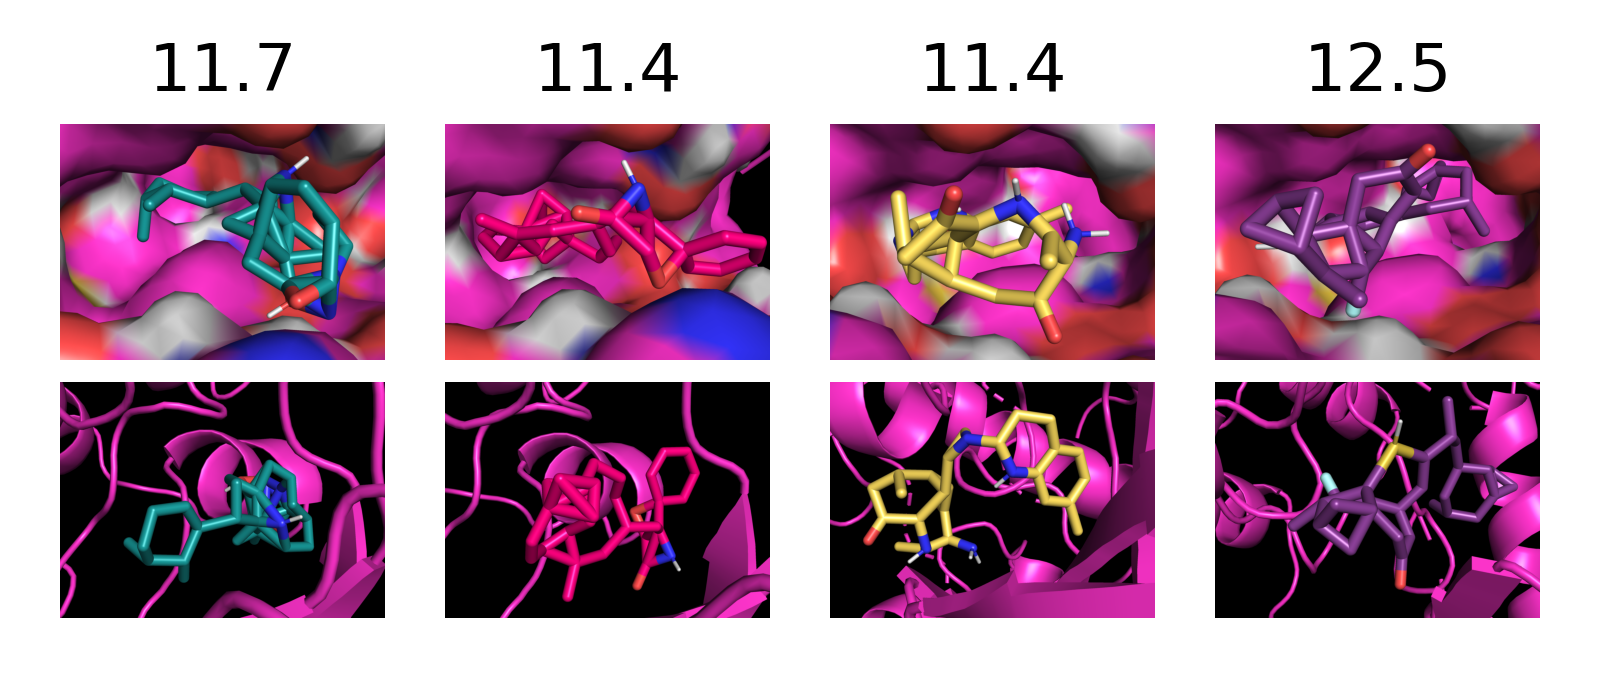
\includegraphics[width=.31\linewidth]{images/mol_vina5.png}
    \label{fig:vina5_grid}}
    \setlength{\belowcaptionskip}{-6pt}
\caption{Generated samples from \alg. For more samples, please refer to \pref{sec:additional_results}. Note that the surfaces and ribbons in (e)-(h) (such as the green objects in (e)) are representations of the target proteins, while the generated small molecules are displayed in the center.
}
\vspace{-2mm}
    \label{fig:compare_images}
\end{figure}

We compare the baselines with our two proposed methods regarding rewards $r$ (Table~\ref{tab:important}). To demonstrate the generated samples' validity (i.e., naturalness), we present several examples in \pref{fig:compare_images}. In \pref{sec:additional_results}, we also include metrics for the validity of samples. 



Overall, \alg\ outperformed the baseline methods (\textbf{Best-of-N}, \textbf{DPS}, and \textbf{SMC}), as evidenced by higher quantiles. Furthermore, for both molecules and images, the samples generated by \alg\ were valid. This suggests that \alg\ can generate high-reward valid samples that \textbf{Best-of-N}, \textbf{DPS}, and \textbf{SMC} often struggle to generate or, in some cases, nearly fail to do.

The relative performance of our \alg-MC and \alg-PM appears to be domain-dependent. Generally, \alg-PM may be more robust since it does not require additional learning (\textit{i.e.}, it directly utilizes reward feedback). The performance of \alg-MC depends on the success of value function learning discussed in \pref{sec:additional}. 

\begin{figure*}[!tb]
    \centering
\begin{subfigure}[c]{0.48\textwidth}
\centering
    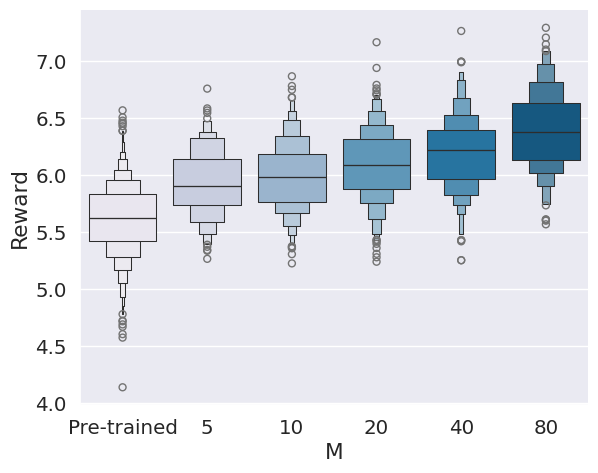
\includegraphics[width=0.60\textwidth]{images/change_K_asthetic.png}
    \caption{Performance of {\alg} as $M$ varies for image generation while optimizing aesthetic score.}
    \label{fig:change_k}
\end{subfigure} 
\begin{subfigure}[c]{0.48\textwidth}
\centering
    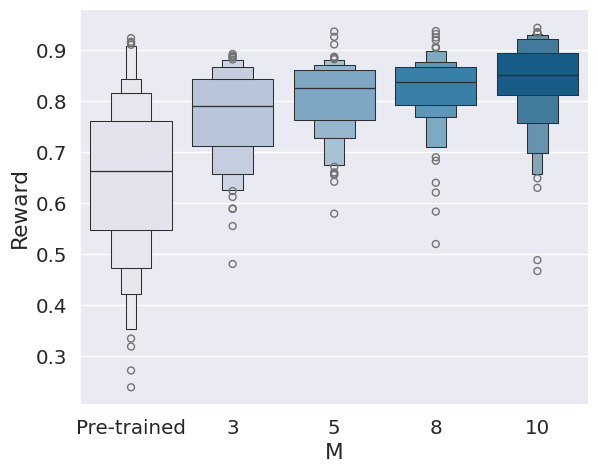
\includegraphics[width=0.60\textwidth]{images/change_M_mol_qed.png}
    \caption{Performance of {\alg} as $M$ varies for molecule generation while optimizing the QED score.}
    \label{fig:change_M_mol}
\end{subfigure} 
 \begin{subfigure}[c]{0.48\textwidth}
 \centering
    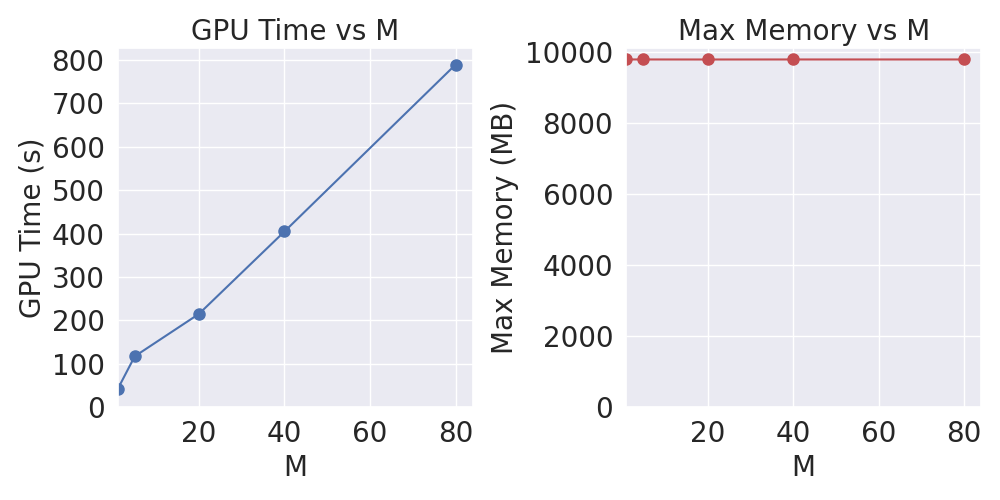
\includegraphics[width=0.80\textwidth]{images/gpu_memory_time_plot_images.png}
    \caption{GPU time and max memory of {\alg} as $M$ varies for image generation (aesthetic scores).  }
    \label{fig:gpu_time_memory}
\end{subfigure}
    \begin{subfigure}[c]{0.48\textwidth}
    \centering
    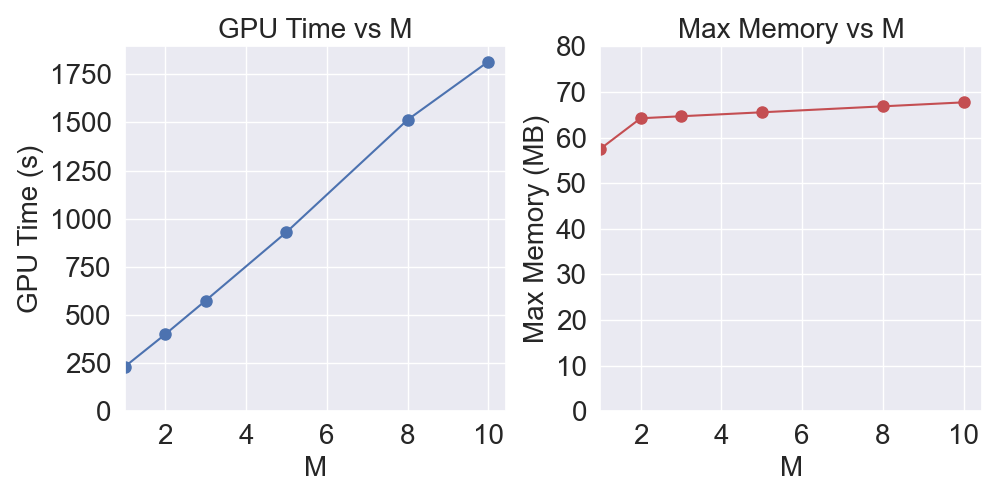
\includegraphics[width=0.80\textwidth]{images/gpu_memory_time_plot.png}
    \caption{GPU time and max memory of {\alg} as $M$ varies for molecule generation (QED). }
    \label{fig:gpu_time_memory2}
\end{subfigure} 
   

\caption{ {Ablation studies with respect to $M$ for \alg. Note \ref{fig:gpu_time_memory} and \ref{fig:gpu_time_memory2} indicate that the computational time does not scale linearly with $M$, whereas memory usage scales linearly.}  }    \label{fig:abletation}
\end{figure*}


\vspace{-2mm}
\paragraph{Ablation studies in terms of the duplication size $M$.} 


We assessed the performance of \alg-PM (when calculating value functions in Line~\ref{line:select2} in a non-parallel manner) along with the computational and memory complexity as $M$ varies. First, across all domains, the performance gradually plateaus as $M$ increases (\pref{fig:change_k} and \ref{fig:change_M_mol}). Second, computational complexity increases linearly with $M$, while memory complexity remains nearly constant (\pref{fig:gpu_time_memory} and \ref{fig:gpu_time_memory2}). This behavior is expected, as previously noted in \pref{sec:inference_time}. The comparison with \textbf{Best-of-N} in Table~\ref{tab:important} is made with this consideration in mind. 



